\documentclass{fizykalab}

% Variables
\def\pomvspace{\vspace{0.3em}}

% Ustawienia strony
\usepackage{lipsum}
\usepackage[margin=3cm]{geometry}
\usepackage{graphicx}
\usepackage{enumitem}
\usepackage{siunitx}
\usepackage{amsmath}
\usepackage{cancel}
\usepackage{makecell}
\usepackage{mathtools}
\setlist{leftmargin=15pt,labelindent=15pt}
\setlist[enumerate]{noitemsep,wide=0pt, leftmargin=*}

% Ustawienia stopki
\usepackage{lastpage}
\usepackage{fancyhdr}
\pagestyle{fancy}
\fancyhf{} % sets both header and footer to nothing
\renewcommand{\headrulewidth}{0pt}
\cfoot{\thepage\ z \pageref{LastPage}}

% Ustawienia do tabelki
\wydzial{IEiT}
\autorjeden{Robert Mesek}
\autordwa{}
\rok{II}
\grupa{8 - L}
\zespol{6}
\temat{Dyfrakcja światła na szczelinie pojedynczej i podwójnej}
\nrcwiczenia{71}
\datawykonania{17.10.2023}
\dataoddaniajeden{}
\zwrotdopoprawy{}
\dataoddaniadwa{}
\datazaliczenia{}

\begin{document}

\maketitle
{\setlength{\parindent}{0pt}
\section*{Ćwiczenie "71": Dyfrakcja}
\subsection*{Cel ćwiczenia}
\par
Celem ćwiczenia jest pomiar natężenia dyfrakcyjnego światła lasera ze szczeliną pojedynczą i podwójną.

\subsection*{Opis ćwiczenia}
\par
Rozkład natężenia światła $I(x)$ wyraża się wzorem
\begin{gather*}
	I(x) = I_0 \left(\frac{\sin (\alpha)}{\alpha}\right)^2 \text{, gdzie } \alpha = \frac{\pi a x}{\lambda} \quad \sin \theta \cong \frac{\pi a x}{\lambda L}
	\tag{1}
\end{gather*}
\begin{flalign*}
	\text{gdzie: } \quad \quad a \ - \  & \text{szerokość szczeliny}            &  & \\
	\lambda \ - \                       & \text{długość fali lasera}            &  & \\
	L \ - \                             & \text{odległość szczeliny od ekranu.} &  & \\
\end{flalign*}

\par
Z funkcji (1) wynikają następujące wzory:

- dla minimów
\begin{equation*}
	x_{min} = m\frac{\lambda L}{a}
	\tag{2}
\end{equation*}

- dla maksimów
\begin{equation*}
	x_{max} = \left(m+\frac{1}{2}\right)\frac{\lambda L}{a}
	\tag{3}
\end{equation*}

W obu wzorach $m$ oznacza numer kolejnego minimum oraz numer kolejnego prążka bocznego.

Stosunki wartości natężenia światła w maksimach bocznych do natężenia maksimum głównego wynoszą:
\begin{equation*}
	\frac{I(x_{max})}{I_0} \cong \frac{1}{\pi^2 \left(m+\frac{1}{2}\right)^2}
	\tag{4}
\end{equation*}

\newpage

\section*{Układ pomiarowy}
\par
W części optycznej układu pomiarowego (Rys. w1):
\begin{itemize}

	\item Laser emitujący światło zielone. Długość fali $\lambda = \SI{530}{\nano\meter}$

	\item Wymienna szczelina (pojedyncza i podwójna)

	\item Fotodioda oraz układ umożliwiający poruszanie ją w kierunku pionowym i poziomym

\end{itemize}
\begin{figure}[!ht]
	\centering
	\vspace{0pt}
	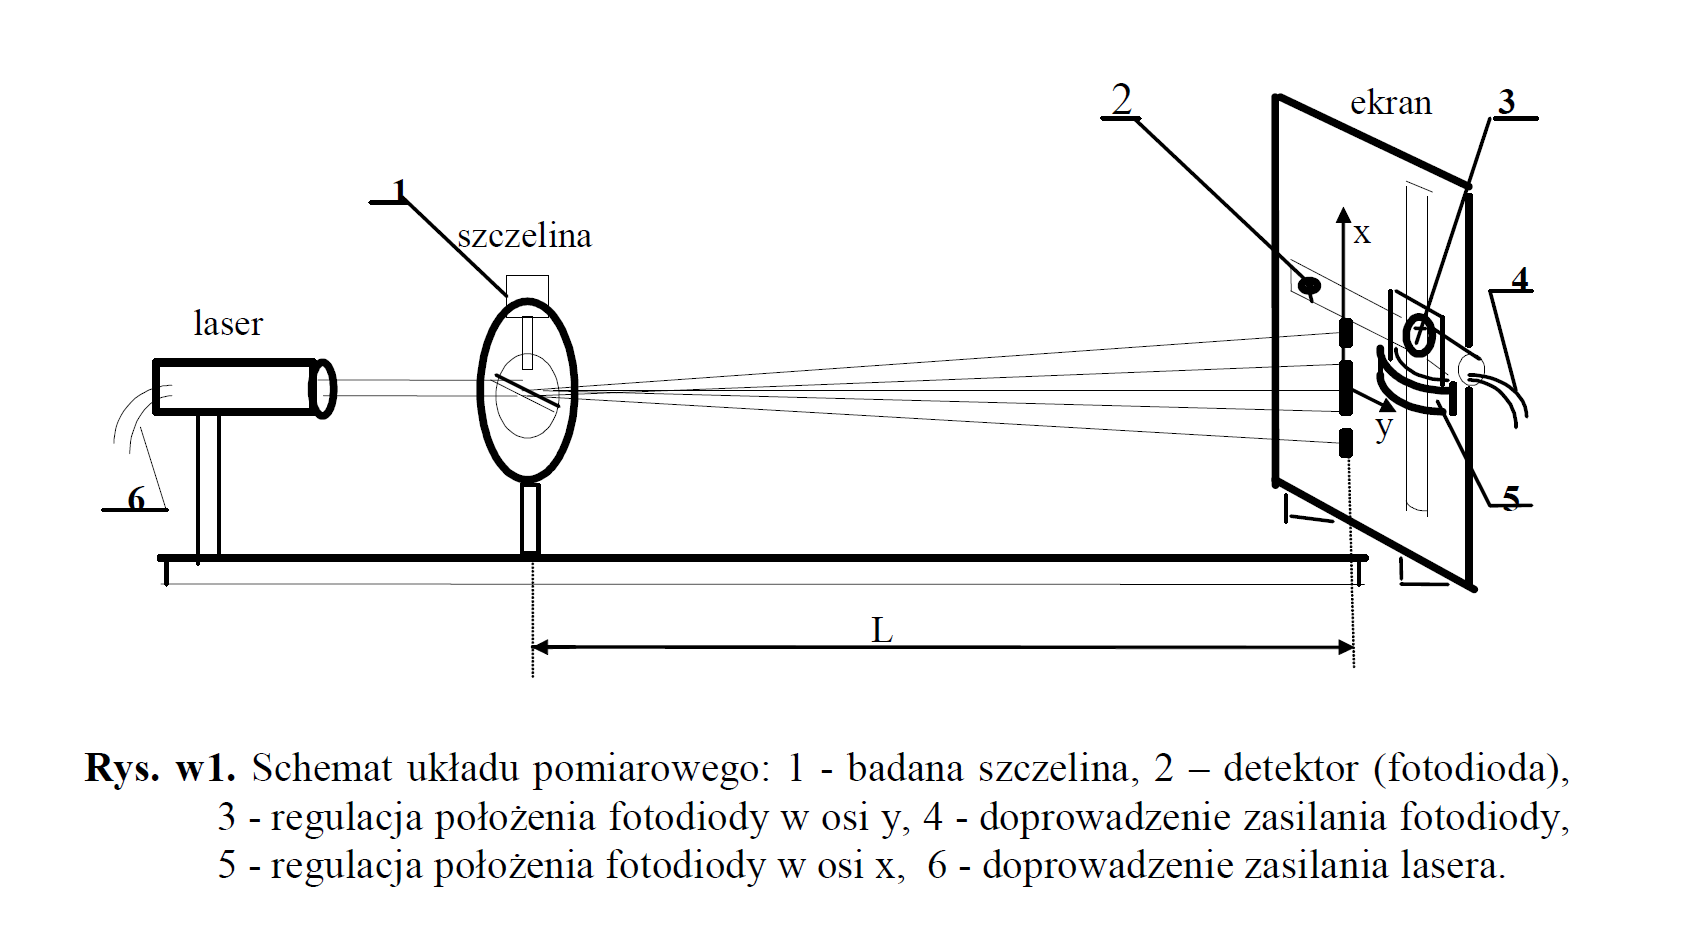
\includegraphics[width=0.9\linewidth]{images/uklad1.png}
\end{figure}
\begin{figure}[!ht]
	\centering
	\vspace{0pt}
	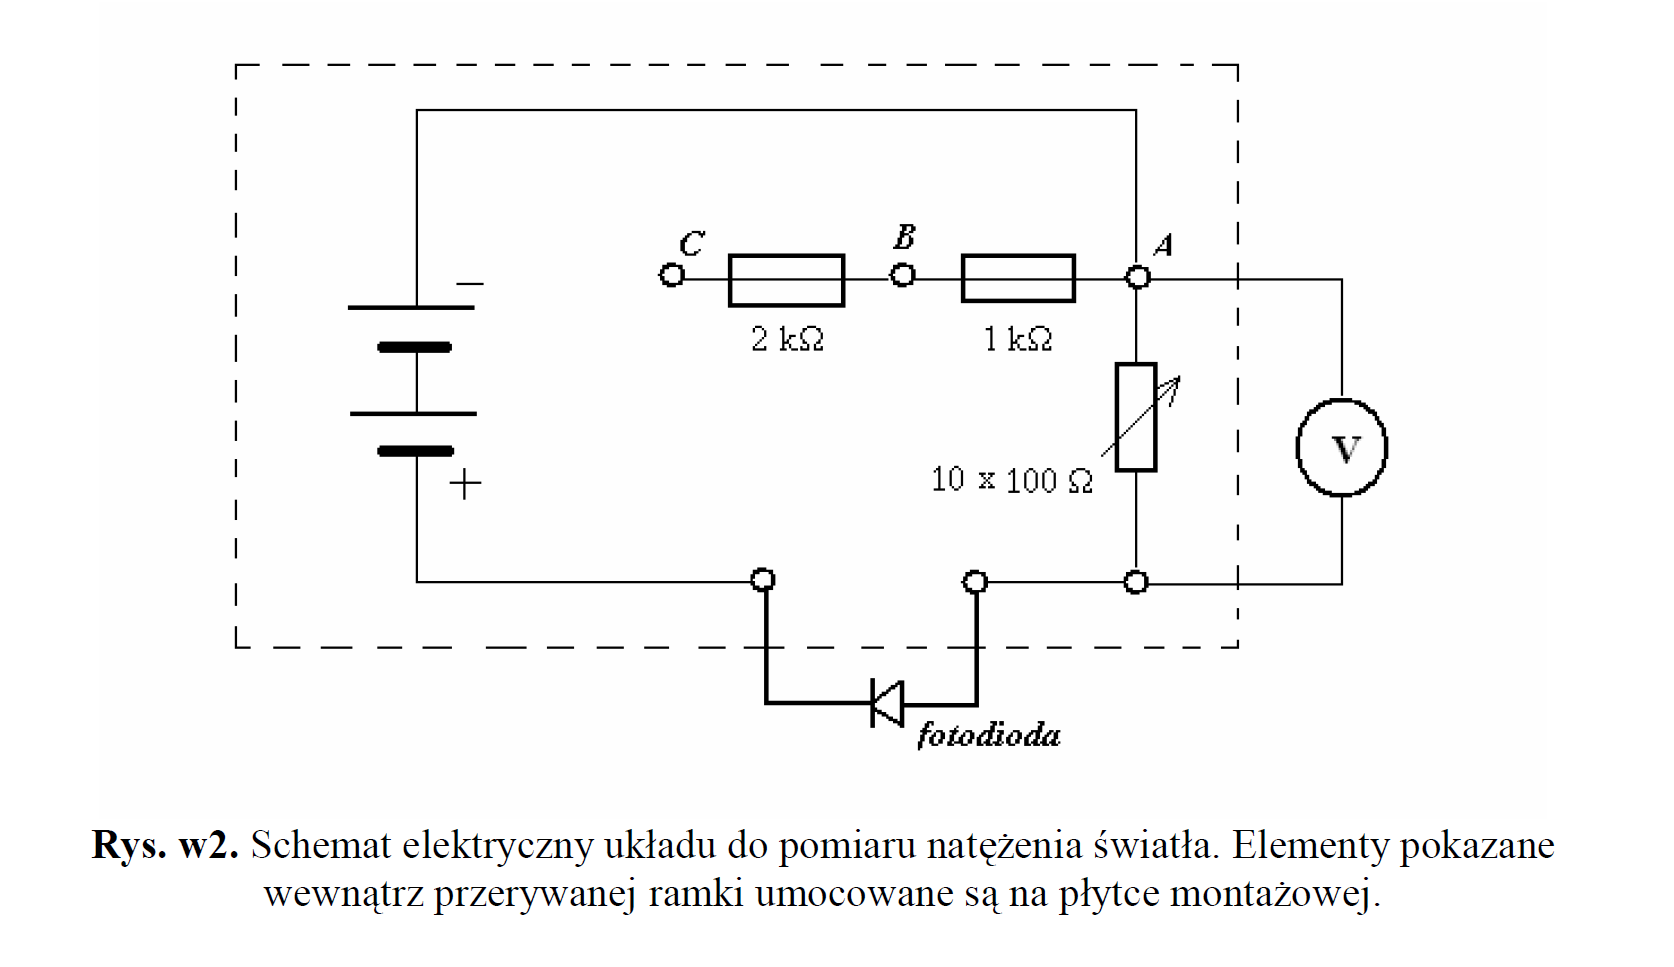
\includegraphics[width=0.9\linewidth]{images/uklad2.png}
\end{figure}

\newpage

\section*{Przebieg doświadczenia}
\par
Uruchamiamy laser oraz obwód mierzący natężenie światła.

Następnie regulujemy położenie fotokomórki, tak aby natężenie światła było maksymalne.

Kolejno zmieniamy jej położenie w płaszczyźnie pionowej co $\Delta x = \SI{0.2}{\milli\meter}$ i odczytujemy wartości natężenia.

Odczytujemy długość fali $\lambda$ wiązki lasera oraz odległość $L$ między szczeliną, a fotodiodą.

\section*{Wyniki pomiarów}
\par
\[ L = \SI{685}{\milli\meter} \pm \SI{1}{\milli\meter}\]

\[ \lambda = \SI{530}{\nano\meter} \]

\begin{figure}[htp]
	\begin{minipage}[t]{0.5\textwidth}
		\centering{Pojedyncza szczelina}

		\begin{minipage}[t]{0.5\textwidth}
				\begin{tabular}{|p{3.5em}|p{3.5em}|}
					\hline
					\textbf{x [mm]} & \textbf{J [j. u.]} \\ \hline\hline
					-5.6 & 0.5 \\ \hline
					-5.4 & 0.3 \\ \hline
					-5.2 & 0.2 \\ \hline
					-5.0 & 0.2 \\ \hline
					-4.8 & 0.3 \\ \hline
					-4.6 & 0.5 \\ \hline
					-4.4 & 0.9 \\ \hline
					-4.2 & 1.3 \\ \hline
					-4.0 & 1.8 \\ \hline
					-3.8 & 2.1 \\ \hline
					-3.6 & 2.2 \\ \hline
					-3.4 & 2.2 \\ \hline
					-3.2 & 1.9 \\ \hline
					-3.0 & 1.4 \\ \hline
					-2.8 & 0.9 \\ \hline
					-2.6 & 0.7 \\ \hline
					-2.4 & 0.9 \\ \hline
					-2.2 & 1.6 \\ \hline
					-2.0 & 3.5 \\ \hline
					-1.8 & 6.4 \\ \hline
					-1.6 & 10.6 \\ \hline
					-1.4 & 15.8 \\ \hline
					-1.2 & 21.6 \\ \hline
					-1.0 & 28.0 \\ \hline
					-0.8 & 34.3 \\ \hline
					-0.6 & 40.2 \\ \hline
					-0.4 & 45.0 \\ \hline
					-0.2 & 48.0 \\ \hline
				\end{tabular}
		\end{minipage}%
		\hfill
		\begin{minipage}[t]{0.5\textwidth}
				\begin{tabular}{|p{3.5em}|p{3.5em}|}
					\hline
					0.0 & 49.6 \\ \hline
					0.2 & 49.4 \\ \hline
					0.4 & 46.9 \\ \hline
					0.6 & 43.6 \\ \hline
					0.8 & 38.6 \\ \hline
					1.0 & 32.2 \\ \hline
					1.2 & 25.7 \\ \hline
					1.4 & 19.1 \\ \hline
					1.6 & 13.4 \\ \hline
					1.8 & 8.9 \\ \hline
					2.0 & 5.3 \\ \hline
					2.2 & 2.5 \\ \hline
					2.4 & 1.0 \\ \hline
					2.6 & 0.5 \\ \hline
					2.8 & 0.5 \\ \hline
					3.0 & 0.9 \\ \hline
					3.2 & 1.4 \\ \hline
					3.4 & 1.9 \\ \hline
					3.6 & 2.1 \\ \hline
					3.8 & 2.1 \\ \hline
					4.0 & 1.9 \\ \hline
					4.2 & 1.5 \\ \hline
					4.4 & 1.0 \\ \hline
					4.6 & 0.6 \\ \hline
					4.8 & 0.3 \\ \hline
					5.0 & 0.2 \\ \hline
					5.2 & 0.1 \\ \hline
					5.4 & 0.2 \\ \hline
					5.6 & 0.4 \\ \hline
				\end{tabular}
		\end{minipage}%
		
		\vspace*{1em}
		\hspace*{-2em}
		\centering{Tabela 1}
		
		\hspace*{\fill}
	\end{minipage}%
	\hfill
	\begin{minipage}[t]{0.5\textwidth}
		\centering{Podwójna szczelina}
		
		\begin{minipage}[t]{0.5\textwidth}
			\begin{tabular}{|p{3.5em}|p{3.5em}|}
				\hline
				\textbf{x [mm]} & \textbf{J [j. u.]} \\ \hline\hline
				-5.6 & 0.3 \\ \hline
				-5.4 & 0.2 \\ \hline
				-5.2 & 0.1 \\ \hline
				-5.0 & 0.1 \\ \hline
				-4.8 & 0.1 \\ \hline
				-4.6 & 0.2 \\ \hline
				-4.4 & 0.4 \\ \hline
				-4.2 & 1.0 \\ \hline
				-4.0 & 2.1 \\ \hline
				-3.8 & 3.2 \\ \hline
				-3.6 & 3.9 \\ \hline
				-3.4 & 3.9 \\ \hline
				-3.2 & 3.0 \\ \hline
				-3.0 & 1.9 \\ \hline
				-2.8 & 1.0 \\ \hline
				-2.6 & 3.8 \\ \hline
				-2.4 & 8.2 \\ \hline
				-2.2 & 13.8 \\ \hline
				-2.0 & 18.8 \\ \hline
				-1.8 & 20.8 \\ \hline
				-1.6 & 18.6 \\ \hline
				-1.4 & 13.2 \\ \hline
				-1.2 & 7.6 \\ \hline
				-1.0 & 4.8 \\ \hline
				-0.8 & 7.4 \\ \hline
				-0.6 & 14.6 \\ \hline
				-0.4 & 23.7 \\ \hline
				-0.2 & 30.7 \\ \hline
			\end{tabular}
		\end{minipage}%
		\hfill
		\begin{minipage}[t]{0.5\textwidth}
			\begin{tabular}{|p{3.5em}|p{3.5em}|}
				\hline
				0.0 & 32.3 \\ \hline
				0.2 & 28.0 \\ \hline
				0.4 & 19.5 \\ \hline
				0.6 & 10.7 \\ \hline
				0.8 & 5.8 \\ \hline
				1.0 & 6.1 \\ \hline
				1.2 & 11.3 \\ \hline
				1.4 & 18.4 \\ \hline
				1.6 & 23.1 \\ \hline
				1.8 & 23.6 \\ \hline
				2.0 & 19.7 \\ \hline
				2.2 & 13.3 \\ \hline
				2.4 & 6.9 \\ \hline
				2.6 & 3.1 \\ \hline
				2.8 & 2.2 \\ \hline
				3.0 & 3.5 \\ \hline
				3.2 & 5.2 \\ \hline
				3.4 & 6.2 \\ \hline
				3.6 & 5.8 \\ \hline
				3.8 & 4.5 \\ \hline
				4.0 & 2.7 \\ \hline
				4.2 & 1.3 \\ \hline
				4.4 & 0.5 \\ \hline
				4.6 & 0.2 \\ \hline
				4.8 & 0.2 \\ \hline
				5.0 & 0.1 \\ \hline
				5.2 & 0.1 \\ \hline
				5.4 & 0.1 \\ \hline
				5.6 & 0.1 \\ \hline
			\end{tabular}
		\end{minipage}%
		
		\vspace*{1em}
		\hspace*{-2em}
		\centering{Tabela 2}
		
		\hspace*{\fill}
		\end{minipage}%
	\hspace*{\fill}
\end{figure}

\newpage

\section*{Opracowanie wyników dla pojedynczej szczeliny}
\begin{figure}[!ht]
	\centering
	\vspace{0pt}
	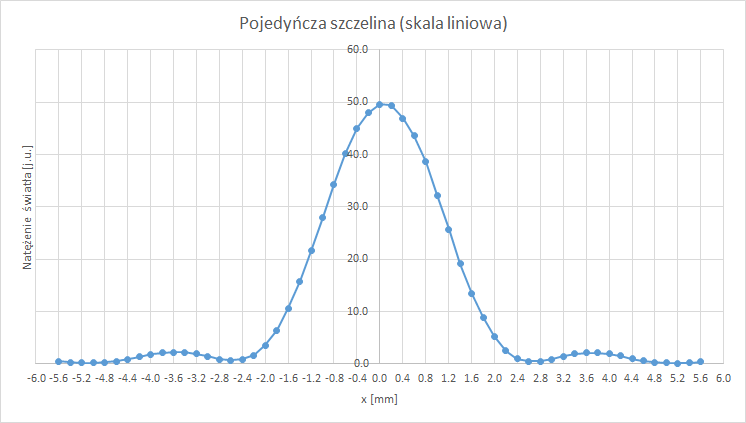
\includegraphics[width=0.9\linewidth]{images/pojedyncza-lin.png}
	\caption{Wykres 1a}
\end{figure}

\begin{figure}[!ht]
	\centering
	\vspace{0pt}
	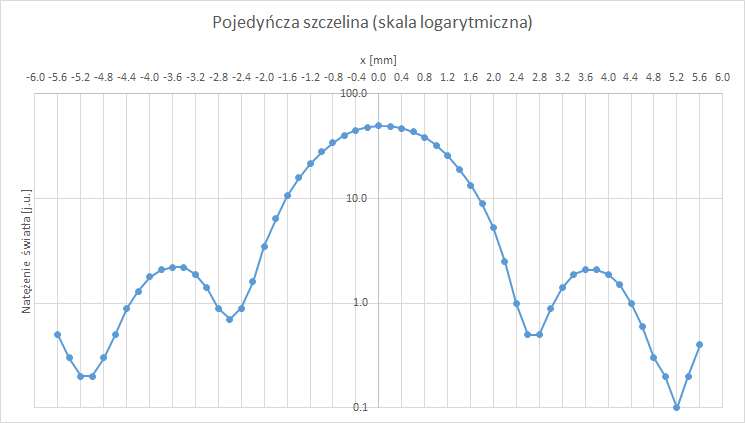
\includegraphics[width=0.9\linewidth]{images/pojedyncza-log.png}
	\caption{Wykres 1b}
\end{figure}

\newpage

\begin{table}[!ht]
	\centering
	\begin{tabular}{|c|c|c|c|c|c|}
		\hline
		\makecell{Element obrazu \\dyfrakcyjnego} & \makecell{Położenie z \\lewej $x_l$ [mm]} & \makecell{Położenie z \\prawej $x_p$ [mm]} & x [mm] & \makecell{Obliczona szerokość \\szczeliny $a$ [mm]} & \makecell{Niepewność \\typu B [mm]} \\ \hline\hline
		1 min & -2.6 & 2.8 & 2.7 & 0.134 & 0.005 \\ \hline
		1 max boczne & -3.6 & 3.8 & 3.7 & 0.147 & 0.003 \\ \hline
		2 min & -5 & 5.2 & 5.1 & 0.142 & 0.003 \\ \hline
	\end{tabular}
	\caption*{Tabela 3 \quad Niepewność typu B ze wzoru (5)}
\end{table}

\par
Tabela 3 przedstawia położenie minimów i maksimów natężenia światła, gdzie:
\[ x = \frac{x_p - x_l}{2} \]
Szerokość szczeliny $a$ jest obliczana ze wzorów (2) i (3).

Średnia wartość a jest równa:
\[\boxed{a = \SI{0.141}{\milli\meter}}\]

Niepewność typu A jest obliczana ze wzoru:
\[ u_a(a) = \sqrt{ \frac{ \sum{(x - \overline{x})^2} }{ N(N-1) } } = \SI{0.004}{\milli\meter} \]

Niepewność typu B jest obliczana z prawa przenoszenia niepewności:
\begin{align*}
u_b(a_{min}) &= \sqrt{\left(\frac{m \lambda}{x_{min}} \cdot u(L)\right)^2 + \left(\frac{-m \lambda L}{x_{min}^2} \cdot u(x)\right)^2}\\
u_b(a_{max}) &= \sqrt{\left(\frac{(m + \frac{1}{2}) \lambda}{x_{max}} \cdot u(L)\right)^2 + \left(\frac{-(m + \frac{1}{2}) \lambda L}{x_{max}^2} \cdot u(x)\right)^2}
\tag{5}
\end{align*} 

gdzie niepewność odległości lasera od fotodiody to $u(L) = 1 \ \text{mm}$, a $u(x) = 0.1 \ \text{mm}$ to niepewność śruby regulującej wysokość fotodiody. 

Średnia niepewność typu B:
\[ u_b(a) = \SI{0.004}{\milli\meter} \]

Niepewność całkowita:
\[ u(a) = \sqrt{u_a(a)^2 + u_b(a)^2} = \SI{0.006}{\milli\meter}\]

Ostatecznie obliczona szerokość szczeliny wynosi:
\[\boxed{a = \SI{0.141}{\milli\meter} \pm \SI{0.006}{\milli\meter}}\]

\newpage

\begin{table}[!ht]
	\centering
	\begin{tabular}{|c|c|c|c|c|}
		\hline
		\makecell{Element obrazu \\dyfrakcyjnego} & \makecell{Natężenie z \\lewej $I_l$ [j.u.]} & \makecell{Natężenie z \\prawej $I_p$ [j.u.]} & \makecell{Natężenie względne \\doświadczalne [j.u.]} & \makecell{Natężenie względne \\teoretyczne [j.u.]} \\ \hline\hline
		1 maksimum boczne & 2.2 & 2.1 & 0.043 & 0.045 \\ \hline
	\end{tabular}
	\caption*{Tabela 4}
\end{table}

Tabela 4 przedstawia natężenie światła dla maksimum bocznego.
Natężenie względne jest obliczona ze wzoru (4), gdzie
\[ I_0 = 49.6 \ \text{[j.u.]} \]


Wartość wyznaczona doświadczalnie jest bardzo zbliżona do wartości teoretycznej:
\[ \boxed{I = 0.043  \ \text{[j.u.]}} \]

Niepewność typu B (w tym przypadku niepewność całkowita) jest obliczana z prawa przenoszenia niepewności:
\[ u(I) = \sqrt{\left(\frac{1}{I_{max}} \cdot u(I_w)\right)^2 + \left(\frac{-I_{min}}{I_{max}^2} \cdot u(I_w)\right)^2} \approx \boxed{0.002 \ \text{[j.u.]}}\]
gdzie $u(I_w)$ to niepewność pomiaru natężenia $= 0.1$ [j.u.]

Ostatecznie obliczone natężenie wynosi:
\[ \boxed{I = 0.043  \ \text{[j.u.]} \pm 0.002 \ \text{[j.u.]}}\]

\subsection*{Wnioski}
\par
Obliczona wartość szczeliny wydaje się prawdopodobną wartością.
Obliczona wartość natężenia jest także w granicy błędu od wartości teoretycznej.

Doświadczenie to dało bardzo dokładne wyniki zgadzające się z przewidywaniami.

\newpage
\section*{Opracowanie wyników dla podwójnej szczeliny}
\begin{figure}[!ht]
	\centering
	\vspace{0pt}
	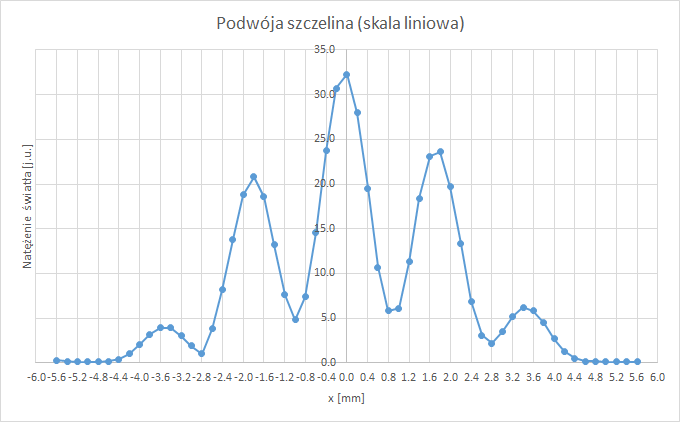
\includegraphics[width=0.9\linewidth]{images/podwojna-lin.png}
	\caption{Wykres 2a}
\end{figure}

\begin{figure}[!ht]
	\centering
	\vspace{0pt}
	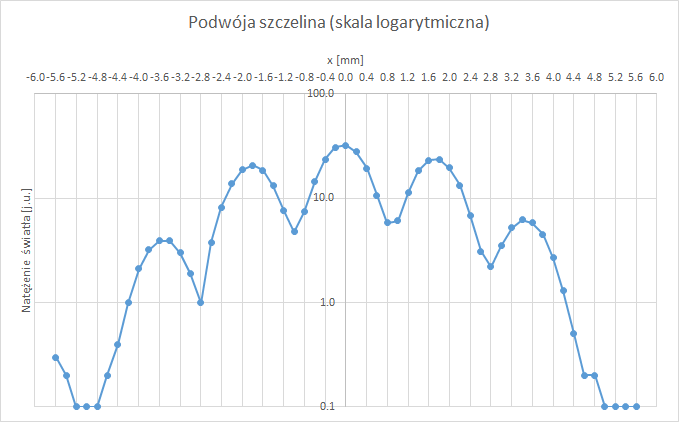
\includegraphics[width=0.9\linewidth]{images/podwojna-log.png}
	\caption{Wykres 2b}
\end{figure}

\newpage

\begin{table}[!ht]
	\centering
	\begin{tabular}{|c|c|c|c|c|c|}
		\hline
		\makecell{Numer \\maksimum (m)} & \makecell{Położenie z \\lewej $x_l$ [mm]} & \makecell{Położenie z \\prawej $x_p$ [mm]} & x [mm] & \makecell{Obliczona szerokość \\szczeliny $a$ [mm]}  & \makecell{Niepewność \\typu B [mm]} \\ \hline\hline
		1 & -1.8 & 1.8 & 1.8 & 0.303 & 0.017 \\ \hline
		2 & -3.4 & 3.4 & 3.4 & 0.267 & 0.008 \\ \hline
	\end{tabular}
	\caption*{Tabela 5 \quad Niepewność typu B ze wzoru (6)}
\end{table}
\par
Tabela 5 przedstawia położenie maksimów natężenia światła, gdzie:
\[ x = \frac{x_p - x_l}{2} \]
Szerokość szczeliny $a$ jest obliczana ze wzorów (2) i (3).

Średnia wartość a jest równa:
\[\boxed{a = \SI{0.285}{\milli\meter}}\]

Niepewność typu A jest obliczana ze wzoru:
\[ u_a(a) = \sqrt{ \frac{ \sum{(x - \overline{x})^2} }{ N(N-1) } } = \SI{0.006}{\milli\meter} \]

Niepewność typu B jest obliczana z prawa przenoszenia niepewności:
\begin{align*}
	u_b(a_{max}) &= \sqrt{\left(\frac{(m + \frac{1}{2}) \lambda}{x_{max}} \cdot u(L)\right)^2 + \left(\frac{-(m + \frac{1}{2}) \lambda L}{x_{max}^2} \cdot u(x)\right)^2}
	\tag{6}
\end{align*} 

gdzie niepewność odległości lasera od fotodiody to $u(L) = 1 \ \text{mm}$, a $u(x) = 0.1 \ \text{mm}$ to niepewność śruby regulującej wysokość fotodiody. 

Średnia niepewność typu B:
\[ u_b(a) = \SI{0.013}{\milli\meter} \]

Niepewność całkowita:
\[ u(a) = \sqrt{u_a(a)^2 + u_b(a)^2} = \SI{0.014}{\milli\meter}\]

Ostatecznie obliczona szerokość szczeliny wynosi:
\[\boxed{a = \SI{0.285}{\milli\meter} \pm \SI{0.014}{\milli\meter}}\]

\paragraph*{Wyznaczenie jakości obrazu interferencyjnego}\mbox{}\newline
Stosunek natężenia w pierwszym minimum do natężenia maksymalnego wynosi:
\[ \frac{I_{min1}}{I_{max}} = \frac{\frac{4.8 + 5.8}{2}}{32.3} = 0.164 \]

\subsection*{Wnioski}
\par
Obliczona wartość szczeliny wydaje się prawdopodobną wartością.

Jakość obrazu interferencyjnego jest dosyć bliska $0$ (odpowiadającego całkowitemu zaniknięciu prążków interferencyjnych).

Doświadczenie to dało dokładne wyniki zgadzające się z przewidywaniami.

\end{document}
